\documentclass[letterpaper,10pt]{article}

\usepackage{titling}
\usepackage{listings}
\usepackage{url}
\usepackage{setspace}
\usepackage{subfig}
\usepackage{sectsty}
\usepackage{pdfpages}
\usepackage{colortbl}
\usepackage{multirow}
\usepackage{relsize}
\usepackage{amsmath}
\usepackage{fancyvrb}
\usepackage{amsmath,amssymb,amsthm,graphicx,xspace}
\usepackage[titlenotnumbered,noend,noline]{algorithm2e}
\usepackage[compact]{titlesec}
\usepackage[default]{droidserif}
\usepackage[T1]{fontenc}
\usepackage{tikz}
\usetikzlibrary{arrows,automata,shapes,trees,matrix,chains,scopes,positioning,calc}
\tikzstyle{block} = [rectangle, draw, fill=blue!20, 
    text width=2.5em, text centered, rounded corners, minimum height=2em]
\tikzstyle{bw} = [rectangle, draw, fill=blue!20, 
    text width=4em, text centered, rounded corners, minimum height=2em]

\definecolor{namerow}{cmyk}{.40,.40,.40,.40}
\definecolor{namecol}{cmyk}{.40,.40,.40,.40}

\let\LaTeXtitle\title
\renewcommand{\title}[1]{\LaTeXtitle{\textsf{#1}}}


\newcommand{\handout}[5]{
  \noindent
  \begin{center}
  \framebox{
    \vbox{
      \hbox to 5.78in { {\bf ECE155: Engineering Design with Embedded Systems } \hfill #2 }
      \vspace{4mm}
      \hbox to 5.78in { {\Large \hfill #4  \hfill} }
      \vspace{2mm}
      \hbox to 5.78in { {\em #3 \hfill} }
    }
  }
  \end{center}
  \vspace*{4mm}
}

\newcommand{\lecture}[3]{\handout{#1}{#2}{#3}{Lecture #1}}
\newcommand{\tuple}[1]{\ensuremath{\left\langle #1 \right\rangle}\xspace}

\addtolength{\oddsidemargin}{-1.000in}
\addtolength{\evensidemargin}{-0.500in}
\addtolength{\textwidth}{2.0in}
\addtolength{\topmargin}{-1.000in}
\addtolength{\textheight}{1.75in}
\addtolength{\parskip}{\baselineskip}
\setlength{\parindent}{0in}
\renewcommand{\baselinestretch}{1.5}
\newcommand{\term}{Spring 2014}

\singlespace


\begin{document}

\lecture{ 31 --- Android IV}{\term}{Jeff Zarnett}

\section*{Android Networking}

We have one more lecture where we're going to look a particularly advanced Android topic: networking. This is not at all necessary for your labs, which is why it did not appear at the start of term along with the rest of the Android material. 

\subsection*{Performing Network Operations}
Before we get started, note that any application that uses the network in Android will need the following permissions.  Code in this section comes from~\cite{android:network1}.
\begin{verbatim}
<uses-permission android:name="android.permission.INTERNET" />
<uses-permission android:name="android.permission.ACCESS_NETWORK_STATE" />
\end{verbatim}

Before connecting to the network, check to make sure that the network is available. The user might have ``Airplane Mode'' turned on and therefore neither mobile internet nor Wi-Fi is available, for example. 

\begin{verbatim}
ConnectivityManager connMgr = (ConnectivityManager) 
        getSystemService(Context.CONNECTIVITY_SERVICE);
    NetworkInfo networkInfo = connMgr.getActiveNetworkInfo();
    if (networkInfo != null && networkInfo.isConnected()) {
    ... // Do useful work
    }
\end{verbatim}

Networks are inherently unreliable and can have unknown latency and bandwidth. If we did network operations in the main activity UI thread, we might get the ``Not Responding'' dialog (remember that from an earlier lecture?). To prevent this from appearing, network operations should take place in a different thread from the UI. How do we do that? In a background task (or asynchronous task), specifically the class \texttt{AsyncTask}. 


\paragraph{AsyncTask} Here is an example of a defined \texttt{AsyncTask}. Explanation follows.

\begin{verbatim}
private class DownloadWebpageTask extends AsyncTask<String, Void, String> {
        @Override
        protected String doInBackground(String... urls) {
              
            // params comes from the execute() call: params[0] is the url.
            try {
                return downloadUrl(urls[0]);
            } catch (IOException e) {
                return "Unable to retrieve web page. URL may be invalid.";
            }
        }
        
        // onPostExecute displays the results of the AsyncTask.
        @Override
        protected void onPostExecute(String result) {
            textView.setText(result);
       }
    }
\end{verbatim}

The \texttt{AsyncTask} we have here is defined as a private class inside a \texttt{MainActivity} but it could be defined as an inner class (\texttt{new AsyncTask<String, Void, String> \{ \ldots \}}) or in its own file. Like a collection, such as \texttt{List}, the \texttt{AsyncTask} takes several parameters inside angle brackets. The first type is the one applicable to the parameter list of \texttt{doInBackground}; the second for \texttt{onProgressUpdate} if any; the third for \texttt{onPostExecute}. Change them as necessary to the applicable types. If you do not need one for some reason, you can put type \texttt{Void} (note capital V).

According to the Android Developer guidelines on the \texttt{AsyncTask}~\cite{asynctask}:
When an asynchronous task is executed, the task goes through 4 steps:

\begin{enumerate}
\item \texttt{onPreExecute()}, invoked on the UI thread before the task is executed. This step is normally used to setup the task, for instance by showing a progress bar in the user interface. Optional; not shown in this example.
\item \texttt{doInBackground(Params...)}, invoked on the background thread immediately after onPreExecute() finishes executing. This step is used to perform background computation that can take a long time. The parameters of the asynchronous task are passed to this step. The result of the computation must be returned by this step and will be passed back to the last step. This step can also use publishProgress(Progress...) to publish one or more units of progress. These values are published on the UI thread, in the \texttt{onProgressUpdate(Progress...)} step. Mandatory (otherwise why use a task?)
\item \texttt{onProgressUpdate(Progress...)}, invoked on the UI thread after a call to publishProgress(Progress...). The timing of the execution is undefined. This method is used to display any form of progress in the user interface while the background computation is still executing. For instance, it can be used to animate a progress bar or show logs in a text field. Optional; not shown in this example.
\item \texttt{onPostExecute(Result)}, invoked on the UI thread after the background computation finishes. The result of the background computation is passed to this step as a parameter.
\end{enumerate}

To actually execute the Download Webpage task, use \texttt{new DownloadWebpageTask().execute(url);} where you fill in the parameters to \texttt{execute} as is appropriate to the \texttt{AsyncTask}. A task can be executed only once; an exception will be thrown if \texttt{execute} is called again. To execute the same thing, create another instance of the task with the \texttt{new} keyword.

A task can be cancelled while it is running by calling \texttt{cancel(boolean)}, but this only makes \texttt{isCancelled()} return true; the \texttt{doInBackground} method should check and see if the task has been cancelled and if so, stop doing what it is doing. Also, after the task is cancelled, instead of \texttt{onPostExecute}, \texttt{onCancelled} is called (also not shown in the example).


\paragraph{Actually Using the Network} 
So after all of that, we are ready to actually use the network!

\begin{verbatim}
// Given a URL, establishes an HttpUrlConnection and retrieves
// the web page content as a InputStream, which it returns as
// a string.
private String downloadUrl(String myurl) throws IOException {
    InputStream is = null;
    // Only display the first 500 characters of the retrieved
    // web page content.
    int len = 500;
        
    try {
        URL url = new URL(myurl);
        HttpURLConnection conn = (HttpURLConnection) url.openConnection();
        conn.setReadTimeout(10000 /* milliseconds */);
        conn.setConnectTimeout(15000 /* milliseconds */);
        conn.setRequestMethod("GET");
        conn.setDoInput(true);
        // Starts the query
        conn.connect();
        int response = conn.getResponseCode();
        Log.d(DEBUG_TAG, "The response is: " + response);
        is = conn.getInputStream();

        // Convert the InputStream into a string
        String contentAsString = readIt(is, len);
        return contentAsString;
        
    // Makes sure that the InputStream is closed after the app is
    // finished using it.
    } finally {
        if (is != null) {
            is.close();
        } 
    }
}

// Reads an InputStream and converts it to a String.
public String readIt(InputStream stream, int len) throws IOException, UnsupportedEncodingException {
    Reader reader = null;
    reader = new InputStreamReader(stream, "UTF-8");        
    char[] buffer = new char[len];
    reader.read(buffer);
    return new String(buffer);
}
\end{verbatim}

The class \texttt{HttpURLConnection} is the key to making the connection over the web. Data can be of any type and it's not necessary to know in advance the length of the data. 

Uses of this class follow a pattern~\cite{httpurl}:
\begin{enumerate}
\item Obtain a new \texttt{HttpURLConnection} by calling \texttt{URL.openConnection()} and casting the result to \texttt{HttpURLConnection}.
\item Prepare the request. The primary property of a request is its URI. Request headers may also include metadata such as credentials, preferred content types, and session cookies.
\item Optionally upload a request body. Instances must be configured with \texttt{setDoOutput(true)} if they include a request body. Transmit data by writing to the stream returned by \texttt{getOutputStream()}.
\item Read the response. Response headers typically include metadata such as the response body's content type and length, modified dates and session cookies. The response body may be read from the stream returned by \texttt{getInputStream()}. If the response has no body, that method returns an empty stream.
\item Disconnect. Once the response body has been read, the \texttt{HttpURLConnection} should be closed by calling \texttt{disconnect()}. Disconnecting releases the resources held by a connection so they may be closed or reused.
\end{enumerate}

Calling \texttt{openConnection()} on a URL with the "https" (HTTP with SSL, security) scheme will return an \texttt{HttpsURLConnection}. We are not going to cover this; for more detail and including things like posting content and authentication, take a look at~\cite{httpurl}.

\subsection*{On Battery Use}
Other than the screen, the next biggest user of battery is likely the wireless radio. The radio for a typical 3G divide has three states:

\begin{enumerate}
	\item \textbf{Full Power}: Uses most power, transfers data at the highest rate.
	\item \textbf{Low Power}: Uses half power.
	\item \textbf{Standby}: Uses minimal power, when no connection is active.
\end{enumerate}

Transition from one state to another is not instant. When the radio is at full power, only if it is idle for five seconds will it transition to the low power state; if it is in low power state, if it is idle for 12 seconds it will go into the standby state. This prevents the situation where the radio is constantly jumping between states due to short pauses. See the diagram below for approximate transition times:

\begin{center}
	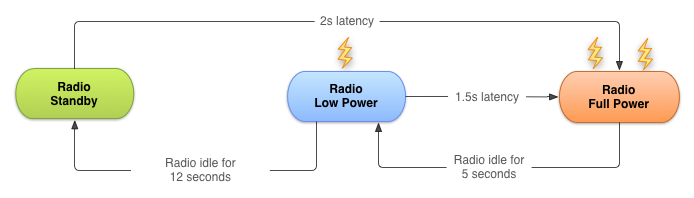
\includegraphics[width=\textwidth]{images/mobile_radio_state_machine.png}
\cite{android:network2}
\end{center}

Creating a new network connection puts the radio in the full power state. If the radio is configured according to the above diagram, a one second transfer is followed by five more seconds of ``tail time'' in the high power state, then twelve seconds in the low power state, before the radio returns to a standby state, for a total of 18 seconds.

If an app transfers unbundled data for 1 second every 18 seconds, it will prevent the radio from ever going to standby, and this will drain a lot of battery. Out of every 60 seconds, 18 will be in the high power state, and the radio will be at the low power state for the remaining 42 seconds.

If we bundled the transfers (i.e., transfer data in bulk), we could save significantly. If we did 3 consecutive seconds of transfer, the radio would be in the high power state for only 8 seconds, and then in the low power state for an additional 12 seconds. The radio would then be idle for the remaining 40 seconds.
\begin{center}
	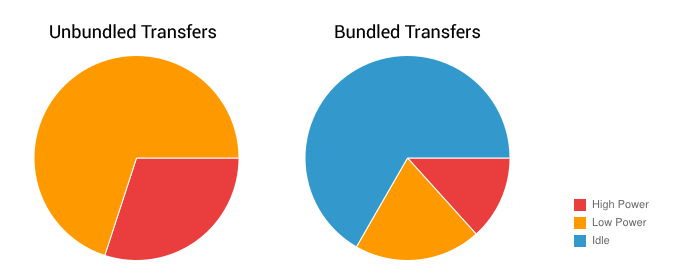
\includegraphics[width=\textwidth]{images/batteryusage.png}

\end{center}

\cite{android:network2}

\subsection*{Cloud Sync}
It's possible to sync your app with the cloud so that user data is not lost even when they reinstall the app or change phones. Google provides a Backup API for small amounts of data (around 1 Megabyte) for storing the user's preferences, high scores, notes etc.

To use the backup service, register for it ( https://developer.android.com/google/backup/signup.html?csw=1 ) and then add the XML tag to your manifest. Then implement the Backup Agent. Example code from~\cite{android:cloudsync}:

\begin{verbatim}
<application android:label="MyApp"
             android:backupAgent="TheBackupAgent">
    ...
    <meta-data android:name="com.google.android.backup.api_key"
    android:value="ABcDe1FGHij2KlmN3oPQRs4TUvW5xYZ" />
    ...
</application>
\end{verbatim}

This registers a backup agent called ``TheBackupAgent'' (change the name as appropriate) which then we implement. Inside the onCreate() method, create a \texttt{BackupHelper}, which in this case looks like this:

\begin{verbatim}
 import android.app.backup.BackupAgentHelper;
 import android.app.backup.FileBackupHelper;


 public class TheBackupAgent extends BackupAgentHelper {
    // The name of the SharedPreferences file
    static final String HIGH_SCORES_FILENAME = "scores";

    // A key to uniquely identify the set of backup data
    static final String FILES_BACKUP_KEY = "myfiles";

    // Allocate a helper and add it to the backup agent
    @Override
    void onCreate() {
        FileBackupHelper helper = new FileBackupHelper(this, HIGH_SCORES_FILENAME);
        addHelper(FILES_BACKUP_KEY, helper);
    }
}
\end{verbatim}

This \texttt{BackupAgentHelper} takes backups of the user's high scores file. If you use \texttt{SharedPreferences} instead, the backup agent helper implementation would look for like this:

\begin{verbatim}
 import android.app.backup.BackupAgentHelper;
 import android.app.backup.SharedPreferencesBackupHelper;

 public class TheBackupAgent extends BackupAgentHelper {
     // The names of the SharedPreferences groups that the application maintains.  These
     // are the same strings that are passed to getSharedPreferences(String, int).
     static final String PREFS_DISPLAY = "displayprefs";
     static final String PREFS_SCORES = "highscores";

     // An arbitrary string used within the BackupAgentHelper implementation to
     // identify the SharedPreferencesBackupHelper's data.
     static final String MY_PREFS_BACKUP_KEY = "myprefs";

     // Simply allocate a helper and install it
     void onCreate() {
         SharedPreferencesBackupHelper helper =
                 new SharedPreferencesBackupHelper(this, PREFS_DISPLAY, PREFS_SCORES);
         addHelper(MY_PREFS_BACKUP_KEY, helper);
     }
 }
\end{verbatim}

To request a backup, just create an instance of the \texttt{BackupManager}, and call its \texttt{dataChanged()} method. This tells the system that data has been changed. If you call \texttt{dataChanged()} more than once before the backup actually takes place, the backup will occur only once (so no extra network traffic will be generated). Restoring from backup happens automatically when the user reinstalls the application, but you can force it with \texttt{requestRestore()}. 

\paragraph{Resolving Sync Conflicts}
It's possible that when you save data to the cloud you end up with conflicts: the user has two or more devices and more than one of them try to save data to the cloud. There are some simple solutions we could follow~\cite{android:cloudsync2}:

\begin{itemize}
\item \textbf{Strategy 1: Newer is better}. A more recent choice should override an older choice. In this case, you would probably choose to store the timestamp in the cloud save data. When resolving the conflict, pick the data set with the most recent timestamp.
\item \textbf{Strategy 2: Value Judgement}. Choose based on some data that can be defined as "best". For example, if the data represents the player's best time in a racing game, keep the best (smallest) time.
\item \textbf{Strategy 3: Merge}. Merge by union. For example, if your data represents the set of levels that player has unlocked, then the resolved data is simply the union of the two conflicting sets. This way, players won't lose any levels they have unlocked.
\end{itemize}

These strategies work if the conflict and data are simple, but we might also have some more complex situations. If we are tracking something important like money, choosing the higher of the two values, for example, is an incorrect solution. Consider the following scenario where we just store the total:

\begin{enumerate}
	\item Starting condition: the user has 0 coins on Device A, 0 on Device B.
	\item Player collects 10 coins on A.
	\item Player collects 15 coins on B.
	\item Device B saves.
	\item Device A saves - conflict detected.
	\item Conflict resolution: choose the largest of the two.
\end{enumerate}
Error occurred: player collected 25 coins but the value of 15 was chosen, so the user has ``lost'' 10 coins.

Idea: Why not send the deltas instead of the values? What if in this situation instead of setting the total, we just send ``+10'' and ``+15''? This works to resolve the scenario here, but Android will send only the most recent update if network connectivity is not available. Imagine that the user collected 5 coins on A while on an airplane (network off) and then in another session, collected another 5 coins. When the synchronization occurs, only the second update will be sent, so only 5 coins will be added to the user's total. Still incorrect.

Solution: store sub-totals per device. Have a separate ``account'' for each device. When the user collects 10 coins on device A, write it into a value for coins collected on A. Then when the time comes to show the overall total, simply sum up the coins collected on A and B.

\bibliographystyle{alpha}
\bibliography{155}


\end{document}